\section{Theorie}
\label{sec:Theorie}
In diesem Versuch wird die Funktionsweise eines \ce{HeNe}-Lasers behandelt. Darauf aufbauend werden
die Stabilitätsbedingung, TEM-Moden, die Polarisationsrichtung und die Wellenlänge des Lasers
genauer betrachtet. Die Begriffe werden im Folgenden näher erläutert.

\subsection{Theoretische Grundlagen und die Stabilitätsbedingung}
Ein Laser (Light Amplification by Stimulated Emission of Radiation) ermöglicht die Erzeugung
von monochromatischem Licht hoher Kohärenz und Intensität. Er setzt sich aus einem aktiven 
Lasermedium, einer Pumpquelle und einem Resonator zusammen. Im Lasermedium werden die Photonen
des Lasers emittiert. 

Es wird ein Zwei-Niveau-System mit den Zuständen ${1}$ und ${2}$ und zugehörigen
Energienieveaus $E_{1}$ und $E_{2}$ betrachtet. Dabei gilt $E_{2}> E_{1}$. Anhand
dieses Systems sollen die möglichen Prozesse erklärt werden, die zu einer Absorption oder 
Emission eines Strahlungsfeldes  $\rho(\nu)$ im Lasermedium führen. Es wird zwischen
drei Prozessen differenziert, die in Abbildung \ref{fig:absorpemiss} skizziert sind.

Durch die Absorption eines Photons der Energie $h \nu = E_{2} - E_{1}$ kann ein Elektron aus dem
Zustand $1$ in den Zustand ${2}$ übergehen. Die Wahrscheinlichkeit $P_{1\rightarrow 2}$ für 
diesen Prozess ist proportional zur spektrale Energiedichte $\rho(\nu)$:
\begin{equation}
	  P_{1\rightarrow 2} = B_{1\rightarrow 2}\cdot\rho(\nu)
\end{equation}
Der Proportionalitätsfaktor $B_{1\rightarrow 2}$ wird als Einsteinkoeffizient der Absorption
bezeichnet. Außerdem kann eine induzierte Emission mit der Wahrscheinlichkeit
\begin{equation}
	  P_{2\rightarrow 1} = B_{2\rightarrow 1}\cdot\rho(\nu)
\end{equation}
stattfinden. Dabei ist  $B_{2\rightarrow1}$ der Einsteinkoeffizient der induzierten Emission.
Das induzierte Photon stimmt in Energie, Phase und Ausbreitungsrichtung mit dem anregenden Photon überein.
Unabhängig vom externen Strahlungsfeld kann auch spontan ein Photon emittiert werden. Die 
Wahrscheinlichkeit für diesen Prozess ergibt sich zu
\begin{equation}
	  P_{s} = A_{2 \rightarrow 1} ,
\end{equation}
wobei $A_{2 \rightarrow 1}$ dem Einsteinkoeffizienten der spontanen Emission entspricht.
Im thermischen Gleichgewicht folgen die Besetzungszahlen $n_{i}$ der Niveaus einer
Boltzmann-Statistik:
\begin{equation}
	n_{i} = \frac{g_{i}n}{Z}\exp\left(-\frac{E_{i}}{k_{B}T}\right)
\end{equation}
Hierbei ist $n$ die Anzahl der Zustände, $g_{i}$ das statistische Gewicht des Zustands ${i}$
und $Z$ die Zustandssumme. Im thermischen Gleichgewicht dominiert somit die Besetzung 
des Grundzustandes. Die Aufgabe des Lasers besteht nun darin,
eine dauerhafte Verstärkung des Strahlungsfeldes zu erzeugen, was durch eine Besetzungsinversion
des Systems realisiert wird. Dies wird durch die Pumpquelle ermöglicht.
Eine Besetzungsinversion ist äquivalent zu der Situation, dass im Medium mehr induzierte 
Emissionen als spontane Emissionen auftreten, was dazu führt, dass das Strahlungsfeld durch
das Medium verstärkt wird.
Weiterhin wird der Resonator dazu verwendet, um den Laufweg der Photonen im Medium zu 
verlängern. Das Prinzip ist in Abbildung \ref{fig:prinzip_laser} dargestellt.
%\begin{figure}
%	  \centering
%	    \includegraphics[width = 0.7\textwidth]{pictures/prinzip_laser.png}
%	        \label{fig:prinzip_laser}
%\end{figure}

Optische Resonatoren sind durch gegenüberliegende Spiegel realisiert, von denen mindestens einer halbdurchlässig ist, um den erzeugten Strahl
auszukoppeln. Verluste an den offenen Rändern der Anordung werden inbesondere durch konfokale Anordnungen minimiert.
In Analogie zum mechanischen Problem eines eingespannten Seiles können nur solche Wellenlängen $\lambda$
im Resonator verstärkt werden, die
folgender Bedingung genügen:
\begin{equation}
	  \lambda = \frac{2 L }{n} \quad n \in  \mathbb{N}.
	    \label{eq:longmoden}
\end{equation}
$L$ ist der Abstand der Spiegel und $n$ wird als longitudinale Mode bezeichent.
Durch die Bedingung \eqref{eq:longmoden} tritt eine Selektion der möglichen Wellenlängen auf. Innerhalb
einer natürlichen spektralen Verteilung, die insbesondere durch den optischen Dopplereffekt hervorgerufen wird, werden nur solche Wellenlängen
verstärkt, die die longitudinale Modenbedingung erfüllen.

Durch Beugungseffekte an Unebenheiten der Spiegel tritt eine Feldverteilung senkrecht zur Resonatorachse auf. Stationäre Intensitätsverteilungen
werden als transversale oder TEM-Moden (\textit{transverse electromagnetic}) bezeichnet. Die Intensität $I_{00}$ der Grundmode $T_{00}$ folgt einer Gaußverteilung:
\begin{equation}
	  I_{00}(d) = I_{0}\exp\left\{- 2\left(\frac{d-d_0}{w}\right)^2\right\}
	    \label{eq: tem00}
\end{equation}
Dabei sind $I_{0}$, $d_0$ und $w$ freie Parameter und $d$ ist der senkrechte Abstand zur
Resonatorachse. Der Parameter $w$ wird auch als Radius
der Fundamentalmode bezeichnet. Die Mode $T_{01}$ kann durch folgende Funktion beschrieben
werden:
\begin{equation} % Ich würde anmerken, dass die T_01 Mode eigentlich symetrisch ist, und nur wegen der Messung asymetrisch ist.
	  I_{01}(d) = I_{0, 1}\exp\left\{- 2\left(\frac{d-d_{0, 1}}{w_{1}}\right)^2\right\} + I_{0, 2}\exp\left\{- 2\left(\frac{d-d_{0,2}}{w_{2}}\right)^2\right\}
	    \label{eq:tem01}
\end{equation}
Dabei wird eine Asymmetrie in der Höhe der beiden Maxima zugelassen (i.A. $I_{0, 1} \neq I_{0, 2}$), die theoretisch nicht
erwartet wird.

Allgemein stellt sich eine stabile Modenverteilung
ein, wenn die folgende Stabilitätbedingung erfüllt ist:
\begin{equation}
	  0 \leq g_1 g_2 \leq 1
	    \label{eq:stabilität}
\end{equation}
Dabei ist
\begin{equation}
	  g_{i} = 1 - L/r_{i}, 
	    \label{eq:spiegelparameter}
\end{equation}
mit den jeweiligen Krümmungsradien $r_{i}$ der Spiegel. 

\subsection{\ce{HeNe}-Laser }
Als Resonatormedium wird beim \ce{HeNe}-Laser ein Gemisch aus $\nicefrac{1}{5}$ Helium und
$\nicefrac{4}{5}$ Neon verwendet, das unter einem Druck von
ca. $\SI{1}{\milli\bar}$ in einem Glaskolben isoliert ist. Das Lasermedium ist Neon, während Helium zum Pumpen verwendet wird.
Die Erzeugung der notwendigen Besetzungsinversion ist in Abbildung~\ref{fig:energieschema} 
illustriert. Durch eine Gasentladung werden
die Heliumatome angeregt, welche wiederum durch Stöße zweiter Art die Neon Atome anregen können. Hierbei sind vorallem die sehr stabilen Zustände
$2^1s$ und $2^3s$ des Helium verantwortlich, deren Anregungsenergie im Rahmen einer natürlichen Linienbreite, die in \ref{fig:energieschema}
eingezeichneten Neon Zustände anregen können. Da die mittlere Lebensdauer des $5s$ Zustandes größer ist als jene des $3p$ Zustandes, tritt die gewünschte
Asymmetrie in den Besetzungszahlen zweier Energienieveaus auf. Stimulierte Emissionsprozesse vom $5s$ in den $3p$ Zustand sind durch die Langlebigkeit
des $5s$-Niveaus pro Zeiteinheit wahrscheinlicher als spontane Emission. Das eingangs beschriebene Zwei-Niveau-System kann eine solche
Asymmetrie nicht erzeugen, da induzierte Absorptionen und Emissionen in gleichem Maße auftreten würden.
Die betreffende Spektrallinie des Übergangs zwischen den beiden Neon-Niveaus liegt mit $\lambda = \SI{632.8}{\nano\meter}$ im sichtbaren
roten Bereich des elektromagnetischen Spektrums.
\begin{figure}
	\centering
	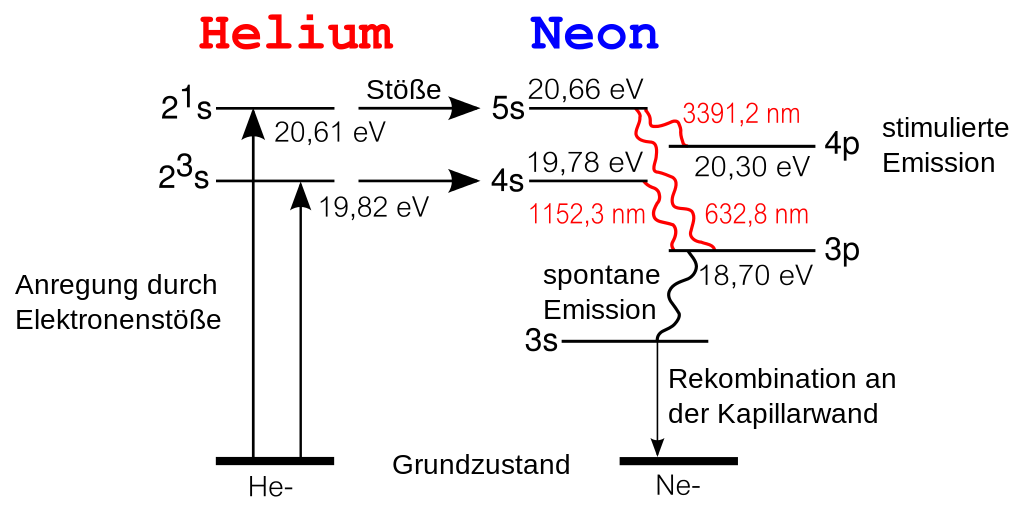
\includegraphics[width = 0.8\textwidth]{pictures/energieschema.png}
	\caption{Darstellung des für den \ce{HeNe}-Laser relevanten Energieschemas \cite{wiki}.}
        \label{fig:energieschema}
\end{figure}
